\documentclass[11pt]{article}
\usepackage[italian]{babel}
\usepackage[utf8]{inputenc}

\usepackage{titlepic} % redefines the \maketitle command to include a picture on your title page, that you provide via the \titlepic command
\usepackage{natbib}
\usepackage{graphicx}
\usepackage{hyperref}
\hypersetup{
    colorlinks=true,
    linkcolor=black,        % color of internal links           %% Andrea
    citecolor=black,        % color of links to bibliography    %% Andrea
    filecolor=blue,         % color of file links               %% Andrea
    urlcolor=blue,          % color of external links           %% Andrea
}

\title{Progetto Interazione Uomo Macchina}
\date{A.A. 2019/2020}
\setcounter{page}{0}

\makeatletter
\def\projectName{Beni culturali}
\let\documentTitle\@title    
\let\academicYear\@date
\makeatother

\begin{document}
\begin{titlepage}
	\centering
    \vspace*{0.5 cm}
    
\includegraphics{images/logosapientini.png}\\[0.75 cm]
%    \textsc{\large Progetto Interazione Uomo Macchina}\\[0.5 cm]
	\textsc{\textit{Università La Sapienza}, Informatica}\\[0.25 cm]
	\textsc{\academicYear}\\[0.5 cm]
	\rule{\linewidth}{0.2 mm} \\[0.4 cm]
	\textsc{\large \documentTitle}\\[0.4 cm]
	%\rule{\linewidth}{0.2 mm} \\[0.4 cm]
	\textsc{\Huge \projectName}\\
	\rule{\linewidth}{0.2 mm} \\[1.5 cm]
	
	\large
	Alessio Berardi, 1796857\\[0.2 cm]
	Andrea Gasparini, 1813486\\[0.2 cm]
    Edoardo Di Paolo, 1728334\\[0.2 cm]
    Enrico Graziani, 1806141\\[0.2 cm]
    Riccardo La Marca, 1795030\\[0.2 cm]
\end{titlepage}

\tableofcontents
\pagebreak

\def\people{20}

\section{Interviste}

\subsection{Introduzione}
Questa sezione riassume i risultati che si sono evinti dalle interviste che abbiamo svolto. Il numero totale di intervistati è di \textbf{\people} persone. Questa fase è stata divisa in due parti poiché ci siamo resi conto che le prime interviste coprivano un campo troppo generico che abbiamo quindi ristretto. I risultati nel dettaglio si riferiscono alle sole informazioni utili raccolte durante la prima fase e a tutte quelle della seconda.

\paragraph{}
Per rendere più efficiente la fase delle interviste abbiamo deciso di dividerci in due gruppi, uno da 2 persone e l'altro da 3 persone, affinché in ogni gruppo ci fosse almeno una persona che aveva come compito quello di prendere appunti riguardo le risposte dateci dagli intervistati.

\subsection{Risultati nel dettaglio}
Andando nel dettaglio, nelle interviste abbiamo toccato, principalmente, i seguenti temi:
    \begin{itemize}
      \item acquisto biglietti (\textit{solo prima fase});
        \item frequenza di visite a musei;
        \item ricerca di informazioni riguardanti musei da visitare;
        \item informazioni riguardanti l'utilizzo o meno delle visite guidate;
        \item informazioni riguardanti sconti universitari (incluse le domeniche gratuite);
        \item informazioni riguardanti l'utilità delle recensioni.
    \end{itemize}
    
\paragraph{}    
Abbiamo chiesto subito come venissero a conoscenza dei musei da visitare e abbiamo scoperto che la maggior parte delle persone si informa grazie ai cartelloni pubblicitari esposti in \textbf{metropolitana, autobus, strade e volantini}. Ovviamente, oltre a questa tipologia di pubblicità, c'è quella che avviene sui \textbf{Social Network}. Relativamente invece all'acquisto dei biglietti si è scoperto che molti li acquistano online in maniera da evitare la fila, invece il restante alla vecchia maniera: cioè al botteghino. In quest'ultimo caso gli intervistati non avevano problemi ad attendere il proprio turno.

\paragraph{}
La maggior parte degli intervistati ha detto di preferire un'\textbf{audioguida} alle \textbf{visite guidate}. Addirittura in molti hanno ammesso di informarsi autonomamente poiché la visita, altrimenti, sarebbe costata di più.
\newline
Gli \textbf{sconti universitari} vengono utilizzati dalla quasi totalità degli studenti intervistati, riguardo le \textbf{domeniche gratuite} invece, la maggior parte ha ammesso di voler utilizzare questa offerta ma, a causa del flusso esagerato di persone, ci rinunciano nella maggior parte dei casi.

\paragraph{}
Le eventuali recensioni di un museo non influenzano la voglia di visitarlo per la maggior parte delle persone. Tutti gli intervistati hanno ammesso di non lasciare alcuna recensione dopo la visita.



\pagebreak
\def\answers{257}

\subsection{Questionario}

Questa sezione riassume i risultati che abbiamo ricevuto dalle risposte al \href{https://docs.google.com/forms/d/1vKzFGCQb5nvyG6it8HfEqZgZ3ioQ6J1_T6eUiTdYIRc/edit}{questionario}. 
Prima di condividere il questionario, abbiamo effettuato un test \textbf{pilota} con 5 utenti per assicurarci che non ci fossero problemi o parti ambigue. Il numero finale di risposte ricevute al questionario è pari a \textbf{\answers}.

\subsubsection{Risultati}
Ai fini del questionario abbiamo raccolto informazioni statistiche, in particolare età e attuale posizione lavorativa. Dai risultati, il \textbf{45\%} è risultato essere studente, il \textbf{34\%} lavoratore, il \textbf{12\%} è studente-lavoratore e il rimanente è disoccupato. Per quanto riguarda l'età, il \textbf{53\%} ha tra i 18-25 anni, il \textbf{19\%} tra i 26 e i 35, l'\textbf{8\%} è minorenne e il restante \textbf{20\%} ha un'età superiore ai 50 anni.

\paragraph{}
Abbiamo scoperto che la metà degli intervistati visita i musei almeno una volta all'anno, mentre solamente in 4 hanno detto di visitarne almeno uno alla settimana.\\
Le visite guidate, dalle risposte, sembrano essere apprezzate e risultano essere utili. 
Si è scoperto che le persone preferiscono andare a visitare un museo in compagnia piuttosto che da soli, ma dalle risposte abbiamo capito che la maggior parte delle persone non trova interessante, o importante, ciò che i propri amici hanno visitato di recente, anche se allo stesso tempo hanno trovato molto utile la possibilità di organizzare visite di gruppo con essi attraverso l'utilizzo dell'applicazione.

\begin{figure}[ht]
    \centering
    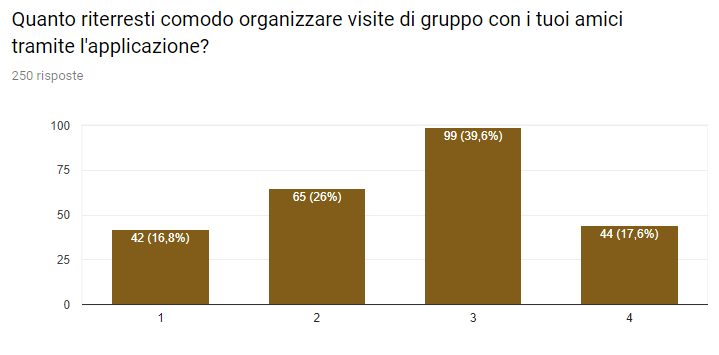
\includegraphics[width=1.0\textwidth]{images/charts-questionario/chart-visite-gruppo.png}
\end{figure}

\begin{figure}[ht]
    \centering
    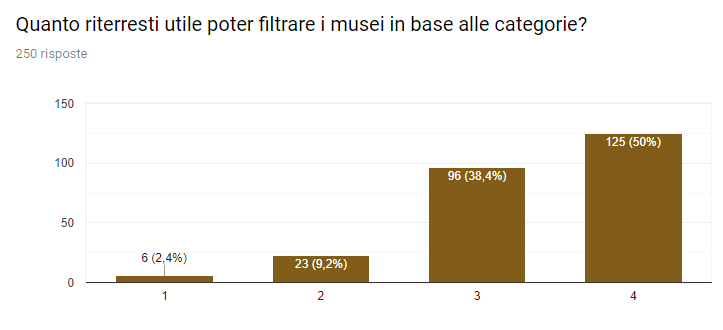
\includegraphics[width=1.0\textwidth]{images/charts-questionario/chart-filtro-categorie.png}
\end{figure}

\paragraph{}
La cosa davvero utile, a quanto pare, è la possibilità di filtrare i musei in base alle categorie che ci sono state segnalate nelle altre risposte.\\
Per quanto riguarda le recensioni, più dell'\textbf{80\%} ha detto di non rilasciarne dopo una visita, anche se comunque la scelta di visitare una mostra rispetto ad un'altra viene molto influenzata dalle recensioni della stessa. Infatti per il \textbf{54\%} delle persone le recensioni sono influenti, ma è importante che siano anche verificate, infatti il \textbf{77\%} ritiene utile poterne verificare l'attendibilità\\
Gli sconti di qualsiasi genere sembrano essere abbastanza utilizzati, a differenza delle visite gratuite.

\begin{figure}[ht]
    \centering
    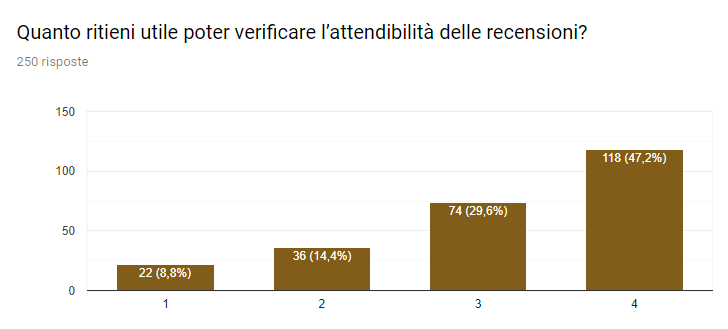
\includegraphics[width=1.0\textwidth]{images/charts-questionario/chart-verifica-recensioni.png}
\end{figure}

\end{document}
